\documentclass[1p]{elsarticle_modified}
%\bibliographystyle{elsarticle-num}

%\usepackage[colorlinks]{hyperref}
%\usepackage{abbrmath_seonhwa} %\Abb, \Ascr, \Acal ,\Abf, \Afrak
\usepackage{amsfonts}
\usepackage{amssymb}
\usepackage{amsmath}
\usepackage{amsthm}
\usepackage{scalefnt}
\usepackage{amsbsy}
\usepackage{kotex}
\usepackage{caption}
\usepackage{subfig}
\usepackage{color}
\usepackage{graphicx}
\usepackage{xcolor} %% white, black, red, green, blue, cyan, magenta, yellow
\usepackage{float}
\usepackage{setspace}
\usepackage{hyperref}

\usepackage{tikz}
\usetikzlibrary{arrows}

\usepackage{multirow}
\usepackage{array} % fixed length table
\usepackage{hhline}

%%%%%%%%%%%%%%%%%%%%%
\makeatletter
\renewcommand*\env@matrix[1][\arraystretch]{%
	\edef\arraystretch{#1}%
	\hskip -\arraycolsep
	\let\@ifnextchar\new@ifnextchar
	\array{*\c@MaxMatrixCols c}}
\makeatother %https://tex.stackexchange.com/questions/14071/how-can-i-increase-the-line-spacing-in-a-matrix
%%%%%%%%%%%%%%%

\usepackage[normalem]{ulem}

\newcommand{\msout}[1]{\ifmmode\text{\sout{\ensuremath{#1}}}\else\sout{#1}\fi}
%SOURCE: \msout is \stkout macro in https://tex.stackexchange.com/questions/20609/strikeout-in-math-mode

\newcommand{\cancel}[1]{
	\ifmmode
	{\color{red}\msout{#1}}
	\else
	{\color{red}\sout{#1}}
	\fi
}

\newcommand{\add}[1]{
	{\color{blue}\uwave{#1}}
}

\newcommand{\replace}[2]{
	\ifmmode
	{\color{red}\msout{#1}}{\color{blue}\uwave{#2}}
	\else
	{\color{red}\sout{#1}}{\color{blue}\uwave{#2}}
	\fi
}

\newcommand{\Sol}{\mathcal{S}} %segment
\newcommand{\D}{D} %diagram
\newcommand{\A}{\mathcal{A}} %arc


%%%%%%%%%%%%%%%%%%%%%%%%%%%%%5 test

\def\sl{\operatorname{\textup{SL}}(2,\Cbb)}
\def\psl{\operatorname{\textup{PSL}}(2,\Cbb)}
\def\quan{\mkern 1mu \triangleright \mkern 1mu}

\theoremstyle{definition}
\newtheorem{thm}{Theorem}[section]
\newtheorem{prop}[thm]{Proposition}
\newtheorem{lem}[thm]{Lemma}
\newtheorem{ques}[thm]{Question}
\newtheorem{cor}[thm]{Corollary}
\newtheorem{defn}[thm]{Definition}
\newtheorem{exam}[thm]{Example}
\newtheorem{rmk}[thm]{Remark}
\newtheorem{alg}[thm]{Algorithm}

\newcommand{\I}{\sqrt{-1}}
\begin{document}

%\begin{frontmatter}
%
%\title{Boundary parabolic representations of knots up to 8 crossings}
%
%%% Group authors per affiliation:
%\author{Yunhi Cho} 
%\address{Department of Mathematics, University of Seoul, Seoul, Korea}
%\ead{yhcho@uos.ac.kr}
%
%
%\author{Seonhwa Kim} %\fnref{s_kim}}
%\address{Center for Geometry and Physics, Institute for Basic Science, Pohang, 37673, Korea}
%\ead{ryeona17@ibs.re.kr}
%
%\author{Hyuk Kim}
%\address{Department of Mathematical Sciences, Seoul National University, Seoul 08826, Korea}
%\ead{hyukkim@snu.ac.kr}
%
%\author{Seokbeom Yoon}
%\address{Department of Mathematical Sciences, Seoul National University, Seoul, 08826,  Korea}
%\ead{sbyoon15@snu.ac.kr}
%
%\begin{abstract}
%We find all boundary parabolic representation of knots up to 8 crossings.
%
%\end{abstract}
%\begin{keyword}
%    \MSC[2010] 57M25 
%\end{keyword}
%
%\end{frontmatter}

%\linenumbers
%\tableofcontents
%
\newcommand\colored[1]{\textcolor{white}{\rule[-0.35ex]{0.8em}{1.4ex}}\kern-0.8em\color{red} #1}%
%\newcommand\colored[1]{\textcolor{white}{ #1}\kern-2.17ex	\textcolor{white}{ #1}\kern-1.81ex	\textcolor{white}{ #1}\kern-2.15ex\color{red}#1	}

{\Large $\underline{12n_{0326}~(K12n_{0326})}$}

\setlength{\tabcolsep}{10pt}
\renewcommand{\arraystretch}{1.6}
\vspace{1cm}\begin{tabular}{m{100pt}>{\centering\arraybackslash}m{274pt}}
\multirow{5}{120pt}{
	\centering
	\includegraphics[width=112pt]{../../../GIT/diagram.site/Diagrams/png/2415_12n_0326.png}\\
\ \ \ A knot diagram\footnotemark}&
\allowdisplaybreaks
\textbf{Linearized knot diagam} \\
\cline{2-2}
 &
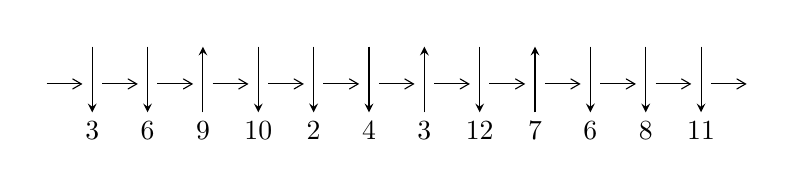
\begin{tikzpicture}[x=20pt, y=17pt]
	% nodes
	\node (C0) at (0, 0) {};
	\node (C1) at (1, 0) {};
	\node (C1U) at (1, +1) {};
	\node (C1D) at (1, -1) {3};

	\node (C2) at (2, 0) {};
	\node (C2U) at (2, +1) {};
	\node (C2D) at (2, -1) {6};

	\node (C3) at (3, 0) {};
	\node (C3U) at (3, +1) {};
	\node (C3D) at (3, -1) {9};

	\node (C4) at (4, 0) {};
	\node (C4U) at (4, +1) {};
	\node (C4D) at (4, -1) {10};

	\node (C5) at (5, 0) {};
	\node (C5U) at (5, +1) {};
	\node (C5D) at (5, -1) {2};

	\node (C6) at (6, 0) {};
	\node (C6U) at (6, +1) {};
	\node (C6D) at (6, -1) {4};

	\node (C7) at (7, 0) {};
	\node (C7U) at (7, +1) {};
	\node (C7D) at (7, -1) {3};

	\node (C8) at (8, 0) {};
	\node (C8U) at (8, +1) {};
	\node (C8D) at (8, -1) {12};

	\node (C9) at (9, 0) {};
	\node (C9U) at (9, +1) {};
	\node (C9D) at (9, -1) {7};

	\node (C10) at (10, 0) {};
	\node (C10U) at (10, +1) {};
	\node (C10D) at (10, -1) {6};

	\node (C11) at (11, 0) {};
	\node (C11U) at (11, +1) {};
	\node (C11D) at (11, -1) {8};

	\node (C12) at (12, 0) {};
	\node (C12U) at (12, +1) {};
	\node (C12D) at (12, -1) {11};
	\node (C13) at (13, 0) {};

	% arrows
	\draw[->,>={angle 60}]
	(C0) edge (C1) (C1) edge (C2) (C2) edge (C3) (C3) edge (C4) (C4) edge (C5) (C5) edge (C6) (C6) edge (C7) (C7) edge (C8) (C8) edge (C9) (C9) edge (C10) (C10) edge (C11) (C11) edge (C12) (C12) edge (C13) ;	\draw[->,>=stealth]
	(C1U) edge (C1D) (C2U) edge (C2D) (C3D) edge (C3U) (C4U) edge (C4D) (C5U) edge (C5D) (C6U) edge (C6D) (C7D) edge (C7U) (C8U) edge (C8D) (C9D) edge (C9U) (C10U) edge (C10D) (C11U) edge (C11D) (C12U) edge (C12D) ;
	\end{tikzpicture} \\
\hhline{~~} \\& 
\textbf{Solving Sequence} \\ \cline{2-2} 
 &
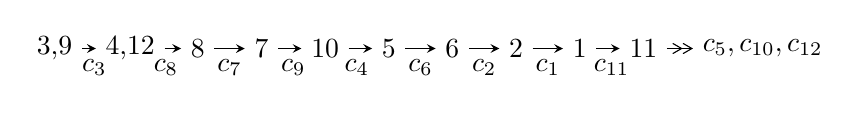
\begin{tikzpicture}[x=23pt, y=7pt]
	% node
	\node (A0) at (-1/8, 0) {3,9};
	\node (A1) at (17/16, 0) {4,12};
	\node (A2) at (17/8, 0) {8};
	\node (A3) at (25/8, 0) {7};
	\node (A4) at (33/8, 0) {10};
	\node (A5) at (41/8, 0) {5};
	\node (A6) at (49/8, 0) {6};
	\node (A7) at (57/8, 0) {2};
	\node (A8) at (65/8, 0) {1};
	\node (A9) at (73/8, 0) {11};
	\node (C1) at (1/2, -1) {$c_{3}$};
	\node (C2) at (13/8, -1) {$c_{8}$};
	\node (C3) at (21/8, -1) {$c_{7}$};
	\node (C4) at (29/8, -1) {$c_{9}$};
	\node (C5) at (37/8, -1) {$c_{4}$};
	\node (C6) at (45/8, -1) {$c_{6}$};
	\node (C7) at (53/8, -1) {$c_{2}$};
	\node (C8) at (61/8, -1) {$c_{1}$};
	\node (C9) at (69/8, -1) {$c_{11}$};
	\node (A10) at (11, 0) {$c_{5},c_{10},c_{12}$};

	% edge
	\draw[->,>=stealth]	
	(A0) edge (A1) (A1) edge (A2) (A2) edge (A3) (A3) edge (A4) (A4) edge (A5) (A5) edge (A6) (A6) edge (A7) (A7) edge (A8) (A8) edge (A9) ;
	\draw[->>,>={angle 60}]	
	(A9) edge (A10);
\end{tikzpicture} \\ 

\end{tabular} \\

\footnotetext{
The image of knot diagram is generated by the software ``\textbf{Draw programme}" developed by Andrew Bartholomew(\url{http://www.layer8.co.uk/maths/draw/index.htm\#Running-draw}), where we modified some parts for our purpose(\url{https://github.com/CATsTAILs/LinksPainter}).
}\phantom \\ \newline 
\centering \textbf{Ideals for irreducible components\footnotemark of $X_{\text{par}}$} 
 
\begin{align*}
I^u_{1}&=\langle 
8.90151\times10^{60} u^{43}+2.21948\times10^{61} u^{42}+\cdots+6.59116\times10^{59} b+1.58663\times10^{62},\\
\phantom{I^u_{1}}&\phantom{= \langle  }-1.69548\times10^{62} u^{43}-4.09643\times10^{62} u^{42}+\cdots+5.93204\times10^{60} a-2.58270\times10^{63},\;u^{44}+3 u^{43}+\cdots+9 u+9\rangle \\
I^u_{2}&=\langle 
- u^{11}+2 u^{10}+u^9-2 u^8-3 u^7+2 u^6+6 u^4-8 u^2+b- u+5,\\
\phantom{I^u_{2}}&\phantom{= \langle  }-3 u^{11}+4 u^9+3 u^8-3 u^7-4 u^6-8 u^5+3 u^4+10 u^3- u^2+a-5 u-1,\\
\phantom{I^u_{2}}&\phantom{= \langle  }u^{12}-2 u^{10}- u^9+2 u^8+2 u^7+2 u^6-2 u^5-5 u^4+u^3+4 u^2-1\rangle \\
I^u_{3}&=\langle 
u^4+u^3-3 u^2+b- u+2,\;u^5+3 u^4-5 u^2+a- u+3,\;u^6+2 u^5-2 u^4-3 u^3+2 u^2+2 u-1\rangle \\
\\
\end{align*}
\raggedright * 3 irreducible components of $\dim_{\mathbb{C}}=0$, with total 62 representations.\\
\footnotetext{All coefficients of polynomials are rational numbers. But the coefficients are sometimes approximated in decimal forms when there is not enough margin.}
\newpage
\renewcommand{\arraystretch}{1}
\centering \section*{I. $I^u_{1}= \langle 8.90\times10^{60} u^{43}+2.22\times10^{61} u^{42}+\cdots+6.59\times10^{59} b+1.59\times10^{62},\;-1.70\times10^{62} u^{43}-4.10\times10^{62} u^{42}+\cdots+5.93\times10^{60} a-2.58\times10^{63},\;u^{44}+3 u^{43}+\cdots+9 u+9 \rangle$}
\flushleft \textbf{(i) Arc colorings}\\
\begin{tabular}{m{7pt} m{180pt} m{7pt} m{180pt} }
\flushright $a_{3}=$&$\begin{pmatrix}1\\0\end{pmatrix}$ \\
\flushright $a_{9}=$&$\begin{pmatrix}0\\u\end{pmatrix}$ \\
\flushright $a_{4}=$&$\begin{pmatrix}1\\- u^2\end{pmatrix}$ \\
\flushright $a_{12}=$&$\begin{pmatrix}28.5817 u^{43}+69.0560 u^{42}+\cdots-332.125 u+435.381\\-13.5052 u^{43}-33.6736 u^{42}+\cdots+226.276 u-240.720\end{pmatrix}$ \\
\flushright $a_{8}=$&$\begin{pmatrix}0.201641 u^{43}+0.460656 u^{42}+\cdots+15.3420 u+12.7889\\33.2391 u^{43}+81.0853 u^{42}+\cdots-419.984 u+535.178\end{pmatrix}$ \\
\flushright $a_{7}=$&$\begin{pmatrix}-33.0375 u^{43}-80.6247 u^{42}+\cdots+435.326 u-522.389\\33.2391 u^{43}+81.0853 u^{42}+\cdots-419.984 u+535.178\end{pmatrix}$ \\
\flushright $a_{10}=$&$\begin{pmatrix}-29.6276 u^{43}-73.3721 u^{42}+\cdots+433.170 u-489.585\\15.3508 u^{43}+38.1625 u^{42}+\cdots-238.731 u+261.946\end{pmatrix}$ \\
\flushright $a_{5}=$&$\begin{pmatrix}-43.7966 u^{43}-107.794 u^{42}+\cdots+594.943 u-730.873\\28.9508 u^{43}+70.9233 u^{42}+\cdots-380.679 u+468.275\end{pmatrix}$ \\
\flushright $a_{6}=$&$\begin{pmatrix}-10.3769 u^{43}-25.2409 u^{42}+\cdots+146.290 u-153.601\\26.2888 u^{43}+64.0967 u^{42}+\cdots-329.420 u+421.797\end{pmatrix}$ \\
\flushright $a_{2}=$&$\begin{pmatrix}27.7669 u^{43}+67.8632 u^{42}+\cdots-348.922 u+460.619\\-6.20167 u^{43}-15.7725 u^{42}+\cdots+127.833 u-117.848\end{pmatrix}$ \\
\flushright $a_{1}=$&$\begin{pmatrix}21.5652 u^{43}+52.0907 u^{42}+\cdots-221.089 u+342.771\\-6.20167 u^{43}-15.7725 u^{42}+\cdots+127.833 u-117.848\end{pmatrix}$ \\
\flushright $a_{11}=$&$\begin{pmatrix}16.2299 u^{43}+39.1273 u^{42}+\cdots-179.657 u+250.432\\-17.7450 u^{43}-43.3750 u^{42}+\cdots+235.483 u-290.417\end{pmatrix}$\\&\end{tabular}
\flushleft \textbf{(ii) Obstruction class $= -1$}\\~\\
\flushleft \textbf{(iii) Cusp Shapes $= -272.965 u^{43}-664.404 u^{42}+\cdots+3337.83 u-4341.43$}\\~\\
\newpage\renewcommand{\arraystretch}{1}
\flushleft \textbf{(iv) u-Polynomials at the component}\newline \\
\begin{tabular}{m{50pt}|m{274pt}}
Crossings & \hspace{64pt}u-Polynomials at each crossing \\
\hline $$\begin{aligned}c_{1}\end{aligned}$$&$\begin{aligned}
&u^{44}+73 u^{43}+\cdots+218241 u+3025
\end{aligned}$\\
\hline $$\begin{aligned}c_{2},c_{5}\end{aligned}$$&$\begin{aligned}
&u^{44}+u^{43}+\cdots+969 u+55
\end{aligned}$\\
\hline $$\begin{aligned}c_{3}\end{aligned}$$&$\begin{aligned}
&u^{44}+3 u^{43}+\cdots+9 u+9
\end{aligned}$\\
\hline $$\begin{aligned}c_{4}\end{aligned}$$&$\begin{aligned}
&u^{44}+u^{43}+\cdots+279 u-9
\end{aligned}$\\
\hline $$\begin{aligned}c_{6}\end{aligned}$$&$\begin{aligned}
&u^{44}-6 u^{43}+\cdots-13 u+1
\end{aligned}$\\
\hline $$\begin{aligned}c_{7}\end{aligned}$$&$\begin{aligned}
&u^{44}+9 u^{42}+\cdots+186673 u+22591
\end{aligned}$\\
\hline $$\begin{aligned}c_{8},c_{11}\end{aligned}$$&$\begin{aligned}
&u^{44}+u^{43}+\cdots+15 u+1
\end{aligned}$\\
\hline $$\begin{aligned}c_{9}\end{aligned}$$&$\begin{aligned}
&u^{44}+8 u^{43}+\cdots+32 u-320
\end{aligned}$\\
\hline $$\begin{aligned}c_{10}\end{aligned}$$&$\begin{aligned}
&u^{44}+6 u^{43}+\cdots-2615847 u-617167
\end{aligned}$\\
\hline $$\begin{aligned}c_{12}\end{aligned}$$&$\begin{aligned}
&u^{44}+33 u^{43}+\cdots-19 u+1
\end{aligned}$\\
\hline
\end{tabular}\\~\\
\newpage\renewcommand{\arraystretch}{1}
\flushleft \textbf{(v) Riley Polynomials at the component}\newline \\
\begin{tabular}{m{50pt}|m{274pt}}
Crossings & \hspace{64pt}Riley Polynomials at each crossing \\
\hline $$\begin{aligned}c_{1}\end{aligned}$$&$\begin{aligned}
&y^{44}-241 y^{43}+\cdots-12809738481 y+9150625
\end{aligned}$\\
\hline $$\begin{aligned}c_{2},c_{5}\end{aligned}$$&$\begin{aligned}
&y^{44}-73 y^{43}+\cdots-218241 y+3025
\end{aligned}$\\
\hline $$\begin{aligned}c_{3}\end{aligned}$$&$\begin{aligned}
&y^{44}-15 y^{43}+\cdots-3087 y+81
\end{aligned}$\\
\hline $$\begin{aligned}c_{4}\end{aligned}$$&$\begin{aligned}
&y^{44}-67 y^{43}+\cdots-87759 y+81
\end{aligned}$\\
\hline $$\begin{aligned}c_{6}\end{aligned}$$&$\begin{aligned}
&y^{44}+2 y^{43}+\cdots-53 y+1
\end{aligned}$\\
\hline $$\begin{aligned}c_{7}\end{aligned}$$&$\begin{aligned}
&y^{44}+18 y^{43}+\cdots+780779441 y+510353281
\end{aligned}$\\
\hline $$\begin{aligned}c_{8},c_{11}\end{aligned}$$&$\begin{aligned}
&y^{44}-33 y^{43}+\cdots+19 y+1
\end{aligned}$\\
\hline $$\begin{aligned}c_{9}\end{aligned}$$&$\begin{aligned}
&y^{44}+10 y^{43}+\cdots-226304 y+102400
\end{aligned}$\\
\hline $$\begin{aligned}c_{10}\end{aligned}$$&$\begin{aligned}
&y^{44}-126 y^{43}+\cdots-7475456601853 y+380895105889
\end{aligned}$\\
\hline $$\begin{aligned}c_{12}\end{aligned}$$&$\begin{aligned}
&y^{44}-33 y^{43}+\cdots+1919 y+1
\end{aligned}$\\
\hline
\end{tabular}\\~\\
\newpage\flushleft \textbf{(vi) Complex Volumes and Cusp Shapes}
$$\begin{array}{c|c|c}  
\text{Solutions to }I^u_{1}& \I (\text{vol} + \sqrt{-1}CS) & \text{Cusp shape}\\
 \hline 
\begin{aligned}
u &= \phantom{-}0.983764 + 0.010812 I \\
a &= \phantom{-}0.776164 + 0.657660 I \\
b &= \phantom{-}0.179807 + 0.453187 I\end{aligned}
 & \phantom{-}3.13780 - 0.62989 I & \phantom{-0.000000 }      -6
0. 10   - 0.363791 I \\ \hline\begin{aligned}
u &= \phantom{-}0.983764 - 0.010812 I \\
a &= \phantom{-}0.776164 - 0.657660 I \\
b &= \phantom{-}0.179807 - 0.453187 I\end{aligned}
 & \phantom{-}3.13780 + 0.62989 I & \phantom{-0.000000 -}     -6
0. 10   + 0.363791 I \\ \hline\begin{aligned}
u &= -0.995926 + 0.212137 I \\
a &= -0.684047 - 0.862199 I \\
b &= \phantom{-}0.385428 - 1.153220 I\end{aligned}
 & \phantom{-}2.87592 - 4.66795 I & \phantom{-0.000000 -}0. + 6.21159 I \\ \hline\begin{aligned}
u &= -0.995926 - 0.212137 I \\
a &= -0.684047 + 0.862199 I \\
b &= \phantom{-}0.385428 + 1.153220 I\end{aligned}
 & \phantom{-}2.87592 + 4.66795 I & \phantom{-0.000000 } 0. - 6.21159 I \\ \hline\begin{aligned}
u &= \phantom{-}0.649512 + 0.810142 I \\
a &= \phantom{-}0.688692 - 1.067530 I \\
b &= -0.58720 - 2.06561 I\end{aligned}
 & -5.69369 + 0.31371 I & -11.24262 + 0. I\phantom{ +0.000000I} \\ \hline\begin{aligned}
u &= \phantom{-}0.649512 - 0.810142 I \\
a &= \phantom{-}0.688692 + 1.067530 I \\
b &= -0.58720 + 2.06561 I\end{aligned}
 & -5.69369 - 0.31371 I & -11.24262 + 0. I\phantom{ +0.000000I} \\ \hline\begin{aligned}
u &= \phantom{-}1.06624\phantom{ +0.000000I} \\
a &= -1.15866\phantom{ +0.000000I} \\
b &= -2.12618\phantom{ +0.000000I}\end{aligned}
 & -8.79014\phantom{ +0.000000I} & -10.1780\phantom{ +0.000000I} \\ \hline\begin{aligned}
u &= \phantom{-}0.972073 + 0.504899 I \\
a &= \phantom{-}0.496608 + 0.409312 I \\
b &= \phantom{-}0.304186 + 0.282887 I\end{aligned}
 & \phantom{-}1.39378 + 1.89935 I & \phantom{-0.000000 } 0 \\ \hline\begin{aligned}
u &= \phantom{-}0.972073 - 0.504899 I \\
a &= \phantom{-}0.496608 - 0.409312 I \\
b &= \phantom{-}0.304186 - 0.282887 I\end{aligned}
 & \phantom{-}1.39378 - 1.89935 I & \phantom{-0.000000 } 0 \\ \hline\begin{aligned}
u &= -1.010890 + 0.500581 I \\
a &= \phantom{-}0.0078406 + 0.1363720 I \\
b &= -0.020428 - 0.546085 I\end{aligned}
 & \phantom{-}0.33573 - 4.72377 I & \phantom{-0.000000 } 0\\
 \hline 
 \end{array}$$\newpage$$\begin{array}{c|c|c}  
\text{Solutions to }I^u_{1}& \I (\text{vol} + \sqrt{-1}CS) & \text{Cusp shape}\\
 \hline 
\begin{aligned}
u &= -1.010890 - 0.500581 I \\
a &= \phantom{-}0.0078406 - 0.1363720 I \\
b &= -0.020428 + 0.546085 I\end{aligned}
 & \phantom{-}0.33573 + 4.72377 I & \phantom{-0.000000 } 0 \\ \hline\begin{aligned}
u &= -0.660411 + 0.938330 I \\
a &= \phantom{-}0.703141 + 0.601609 I \\
b &= -0.80986 + 1.28827 I\end{aligned}
 & -2.22612 + 0.56711 I & \phantom{-0.000000 } 0 \\ \hline\begin{aligned}
u &= -0.660411 - 0.938330 I \\
a &= \phantom{-}0.703141 - 0.601609 I \\
b &= -0.80986 - 1.28827 I\end{aligned}
 & -2.22612 - 0.56711 I & \phantom{-0.000000 } 0 \\ \hline\begin{aligned}
u &= \phantom{-}1.057930 + 0.650598 I \\
a &= -0.899709 + 0.653233 I \\
b &= \phantom{-}0.83419 + 2.06344 I\end{aligned}
 & -4.35874 + 5.22725 I & \phantom{-0.000000 } 0 \\ \hline\begin{aligned}
u &= \phantom{-}1.057930 - 0.650598 I \\
a &= -0.899709 - 0.653233 I \\
b &= \phantom{-}0.83419 - 2.06344 I\end{aligned}
 & -4.35874 - 5.22725 I & \phantom{-0.000000 } 0 \\ \hline\begin{aligned}
u &= -0.820834 + 0.933777 I \\
a &= -1.161680 - 0.646565 I \\
b &= \phantom{-}0.541938 - 1.130020 I\end{aligned}
 & -15.6870 - 0.6720 I & \phantom{-0.000000 } 0 \\ \hline\begin{aligned}
u &= -0.820834 - 0.933777 I \\
a &= -1.161680 + 0.646565 I \\
b &= \phantom{-}0.541938 + 1.130020 I\end{aligned}
 & -15.6870 + 0.6720 I & \phantom{-0.000000 } 0 \\ \hline\begin{aligned}
u &= -1.050360 + 0.680819 I \\
a &= -0.518016 - 0.831087 I \\
b &= \phantom{-}0.75737 - 2.31620 I\end{aligned}
 & -0.97641 - 6.41642 I & \phantom{-0.000000 } 0 \\ \hline\begin{aligned}
u &= -1.050360 - 0.680819 I \\
a &= -0.518016 + 0.831087 I \\
b &= \phantom{-}0.75737 + 2.31620 I\end{aligned}
 & -0.97641 + 6.41642 I & \phantom{-0.000000 } 0 \\ \hline\begin{aligned}
u &= -0.484046 + 0.563326 I \\
a &= \phantom{-}0.363504 + 0.096522 I \\
b &= -0.396795 + 0.188011 I\end{aligned}
 & -1.234310 + 0.383646 I & -8.59433 - 2.13005 I\\
 \hline 
 \end{array}$$\newpage$$\begin{array}{c|c|c}  
\text{Solutions to }I^u_{1}& \I (\text{vol} + \sqrt{-1}CS) & \text{Cusp shape}\\
 \hline 
\begin{aligned}
u &= -0.484046 - 0.563326 I \\
a &= \phantom{-}0.363504 - 0.096522 I \\
b &= -0.396795 - 0.188011 I\end{aligned}
 & -1.234310 - 0.383646 I & -8.59433 + 2.13005 I \\ \hline\begin{aligned}
u &= \phantom{-}0.804579 + 0.967738 I \\
a &= -0.798757 - 0.489353 I \\
b &= -0.453409 - 0.664044 I\end{aligned}
 & -11.28860 - 0.64983 I & \phantom{-0.000000 } 0 \\ \hline\begin{aligned}
u &= \phantom{-}0.804579 - 0.967738 I \\
a &= -0.798757 + 0.489353 I \\
b &= -0.453409 + 0.664044 I\end{aligned}
 & -11.28860 + 0.64983 I & \phantom{-0.000000 } 0 \\ \hline\begin{aligned}
u &= -0.652932 + 0.251845 I \\
a &= \phantom{-}0.54350 + 1.32899 I \\
b &= \phantom{-}0.639215 + 0.232761 I\end{aligned}
 & \phantom{-}1.23289 - 4.62902 I & -5.84465 + 4.14155 I \\ \hline\begin{aligned}
u &= -0.652932 - 0.251845 I \\
a &= \phantom{-}0.54350 - 1.32899 I \\
b &= \phantom{-}0.639215 - 0.232761 I\end{aligned}
 & \phantom{-}1.23289 + 4.62902 I & -5.84465 - 4.14155 I \\ \hline\begin{aligned}
u &= \phantom{-}0.670851\phantom{ +0.000000I} \\
a &= \phantom{-}2.40416\phantom{ +0.000000I} \\
b &= -2.11628\phantom{ +0.000000I}\end{aligned}
 & -10.5877\phantom{ +0.000000I} & \phantom{-}8.90790\phantom{ +0.000000I} \\ \hline\begin{aligned}
u &= -1.048190 + 0.837144 I \\
a &= \phantom{-}0.484292 + 1.026390 I \\
b &= -0.06811 + 2.25749 I\end{aligned}
 & -14.9574 - 5.9017 I & \phantom{-0.000000 } 0 \\ \hline\begin{aligned}
u &= -1.048190 - 0.837144 I \\
a &= \phantom{-}0.484292 - 1.026390 I \\
b &= -0.06811 - 2.25749 I\end{aligned}
 & -14.9574 + 5.9017 I & \phantom{-0.000000 } 0 \\ \hline\begin{aligned}
u &= -0.651141\phantom{ +0.000000I} \\
a &= \phantom{-}1.08862\phantom{ +0.000000I} \\
b &= -0.346698\phantom{ +0.000000I}\end{aligned}
 & -1.21790\phantom{ +0.000000I} & -7.98940\phantom{ +0.000000I} \\ \hline\begin{aligned}
u &= \phantom{-}1.060320 + 0.850355 I \\
a &= -0.636937 - 0.700265 I \\
b &= -0.449291 - 0.476529 I\end{aligned}
 & -10.46950 + 7.35029 I & \phantom{-0.000000 } 0\\
 \hline 
 \end{array}$$\newpage$$\begin{array}{c|c|c}  
\text{Solutions to }I^u_{1}& \I (\text{vol} + \sqrt{-1}CS) & \text{Cusp shape}\\
 \hline 
\begin{aligned}
u &= \phantom{-}1.060320 - 0.850355 I \\
a &= -0.636937 + 0.700265 I \\
b &= -0.449291 + 0.476529 I\end{aligned}
 & -10.46950 - 7.35029 I & \phantom{-0.000000 } 0 \\ \hline\begin{aligned}
u &= \phantom{-}0.919976 + 1.023950 I \\
a &= \phantom{-}0.546144 - 0.830602 I \\
b &= -0.86441 - 1.77933 I\end{aligned}
 & -4.52279 + 6.69405 I & \phantom{-0.000000 } 0 \\ \hline\begin{aligned}
u &= \phantom{-}0.919976 - 1.023950 I \\
a &= \phantom{-}0.546144 + 0.830602 I \\
b &= -0.86441 + 1.77933 I\end{aligned}
 & -4.52279 - 6.69405 I & \phantom{-0.000000 } 0 \\ \hline\begin{aligned}
u &= -0.582341\phantom{ +0.000000I} \\
a &= -1.15614\phantom{ +0.000000I} \\
b &= -1.48403\phantom{ +0.000000I}\end{aligned}
 & -2.44265\phantom{ +0.000000I} & \phantom{-}5.79850\phantom{ +0.000000I} \\ \hline\begin{aligned}
u &= -0.545744\phantom{ +0.000000I} \\
a &= \phantom{-}1.19923\phantom{ +0.000000I} \\
b &= -3.94886\phantom{ +0.000000I}\end{aligned}
 & -6.50431\phantom{ +0.000000I} & -21.3880\phantom{ +0.000000I} \\ \hline\begin{aligned}
u &= -0.70181 + 1.29455 I \\
a &= -0.760731 - 0.722556 I \\
b &= \phantom{-}0.44712 - 1.62807 I\end{aligned}
 & -16.5470 + 6.4689 I & \phantom{-0.000000 } 0 \\ \hline\begin{aligned}
u &= -0.70181 - 1.29455 I \\
a &= -0.760731 + 0.722556 I \\
b &= \phantom{-}0.44712 + 1.62807 I\end{aligned}
 & -16.5470 - 6.4689 I & \phantom{-0.000000 } 0 \\ \hline\begin{aligned}
u &= -1.23575 + 0.88133 I \\
a &= \phantom{-}0.521632 + 0.894334 I \\
b &= -0.61086 + 2.31759 I\end{aligned}
 & -14.7157 - 14.1505 I & \phantom{-0.000000 } 0 \\ \hline\begin{aligned}
u &= -1.23575 - 0.88133 I \\
a &= \phantom{-}0.521632 - 0.894334 I \\
b &= -0.61086 - 2.31759 I\end{aligned}
 & -14.7157 + 14.1505 I & \phantom{-0.000000 } 0 \\ \hline\begin{aligned}
u &= \phantom{-}0.298088 + 0.083893 I \\
a &= -2.74531 + 3.08989 I \\
b &= \phantom{-}0.155988 + 0.909226 I\end{aligned}
 & \phantom{-}0.144274 + 0.902896 I & -6.75614 - 2.40130 I\\
 \hline 
 \end{array}$$\newpage$$\begin{array}{c|c|c}  
\text{Solutions to }I^u_{1}& \I (\text{vol} + \sqrt{-1}CS) & \text{Cusp shape}\\
 \hline 
\begin{aligned}
u &= \phantom{-}0.298088 - 0.083893 I \\
a &= -2.74531 - 3.08989 I \\
b &= \phantom{-}0.155988 - 0.909226 I\end{aligned}
 & \phantom{-}0.144274 - 0.902896 I & -6.75614 + 2.40130 I \\ \hline\begin{aligned}
u &= \phantom{-}1.34675 + 1.16951 I \\
a &= -0.459956 + 0.487071 I \\
b &= \phantom{-}0.60751 + 1.79387 I\end{aligned}
 & -3.83190 + 1.09484 I & \phantom{-0.000000 } 0 \\ \hline\begin{aligned}
u &= \phantom{-}1.34675 - 1.16951 I \\
a &= -0.459956 - 0.487071 I \\
b &= \phantom{-}0.60751 - 1.79387 I\end{aligned}
 & -3.83190 - 1.09484 I & \phantom{-0.000000 } 0 \\ \hline\begin{aligned}
u &= -1.82155\phantom{ +0.000000I} \\
a &= \phantom{-}0.356733\phantom{ +0.000000I} \\
b &= -2.16268\phantom{ +0.000000I}\end{aligned}
 & -2.68064\phantom{ +0.000000I} & \phantom{-0.000000 } 0\\
 \hline 
 \end{array}$$\newpage\newpage\renewcommand{\arraystretch}{1}
\centering \section*{II. $I^u_{2}= \langle - u^{11}+2 u^{10}+\cdots+b+5,\;-3 u^{11}+4 u^9+\cdots+a-1,\;u^{12}-2 u^{10}+\cdots+4 u^2-1 \rangle$}
\flushleft \textbf{(i) Arc colorings}\\
\begin{tabular}{m{7pt} m{180pt} m{7pt} m{180pt} }
\flushright $a_{3}=$&$\begin{pmatrix}1\\0\end{pmatrix}$ \\
\flushright $a_{9}=$&$\begin{pmatrix}0\\u\end{pmatrix}$ \\
\flushright $a_{4}=$&$\begin{pmatrix}1\\- u^2\end{pmatrix}$ \\
\flushright $a_{12}=$&$\begin{pmatrix}3 u^{11}-4 u^9-3 u^8+3 u^7+4 u^6+8 u^5-3 u^4-10 u^3+u^2+5 u+1\\u^{11}-2 u^{10}- u^9+2 u^8+3 u^7-2 u^6-6 u^4+8 u^2+u-5\end{pmatrix}$ \\
\flushright $a_{8}=$&$\begin{pmatrix}u^{11}+2 u^{10}-2 u^9-5 u^8+5 u^6+6 u^5+3 u^4-8 u^3-9 u^2+5 u+5\\-2 u^{10}+3 u^8+2 u^7-3 u^6-3 u^5-5 u^4+3 u^3+8 u^2- u-5\end{pmatrix}$ \\
\flushright $a_{7}=$&$\begin{pmatrix}u^{11}+4 u^{10}+\cdots+6 u+10\\-2 u^{10}+3 u^8+2 u^7-3 u^6-3 u^5-5 u^4+3 u^3+8 u^2- u-5\end{pmatrix}$ \\
\flushright $a_{10}=$&$\begin{pmatrix}19 u^{11}+6 u^{10}+\cdots+46 u+22\\-10 u^{11}- u^{10}+\cdots-23 u-6\end{pmatrix}$ \\
\flushright $a_{5}=$&$\begin{pmatrix}-22 u^{11}-19 u^{10}+\cdots-68 u-45\\6 u^{11}+10 u^{10}+\cdots+23 u+23\end{pmatrix}$ \\
\flushright $a_{6}=$&$\begin{pmatrix}u^{11}+3 u^{10}-2 u^9-7 u^8- u^7+7 u^6+8 u^5+5 u^4-10 u^3-15 u^2+6 u+9\\- u^{10}+2 u^8+u^7-2 u^6-2 u^5-2 u^4+2 u^3+5 u^2- u-4\end{pmatrix}$ \\
\flushright $a_{2}=$&$\begin{pmatrix}6 u^{11}+9 u^{10}+\cdots+23 u+22\\- u^{11}-4 u^{10}+\cdots-6 u-11\end{pmatrix}$ \\
\flushright $a_{1}=$&$\begin{pmatrix}5 u^{11}+5 u^{10}+\cdots+17 u+11\\- u^{11}-4 u^{10}+\cdots-6 u-11\end{pmatrix}$ \\
\flushright $a_{11}=$&$\begin{pmatrix}- u^{11}- u^{10}+3 u^9+2 u^8-2 u^7-4 u^6-3 u^5+9 u^3+u^2-6 u-2\\2 u^{11}-3 u^9-2 u^8+3 u^7+3 u^6+5 u^5-3 u^4-8 u^3+u^2+6 u\end{pmatrix}$\\&\end{tabular}
\flushleft \textbf{(ii) Obstruction class $= 1$}\\~\\
\flushleft \textbf{(iii) Cusp Shapes $= -16 u^{11}-7 u^{10}+23 u^9+24 u^8-14 u^7-27 u^6-48 u^5- u^4+62 u^3+12 u^2-37 u-17$}\\~\\
\newpage\renewcommand{\arraystretch}{1}
\flushleft \textbf{(iv) u-Polynomials at the component}\newline \\
\begin{tabular}{m{50pt}|m{274pt}}
Crossings & \hspace{64pt}u-Polynomials at each crossing \\
\hline $$\begin{aligned}c_{1}\end{aligned}$$&$\begin{aligned}
&u^{12}-12 u^{11}+\cdots+4 u^2+1
\end{aligned}$\\
\hline $$\begin{aligned}c_{2}\end{aligned}$$&$\begin{aligned}
&u^{12}+8 u^{11}+\cdots+4 u+1
\end{aligned}$\\
\hline $$\begin{aligned}c_{3}\end{aligned}$$&$\begin{aligned}
&u^{12}-2 u^{10}- u^9+2 u^8+2 u^7+2 u^6-2 u^5-5 u^4+u^3+4 u^2-1
\end{aligned}$\\
\hline $$\begin{aligned}c_{4}\end{aligned}$$&$\begin{aligned}
&u^{12}-4 u^{10}+u^9+5 u^8-2 u^7-2 u^6+2 u^5-2 u^4- u^3+2 u^2-1
\end{aligned}$\\
\hline $$\begin{aligned}c_{5}\end{aligned}$$&$\begin{aligned}
&u^{12}-8 u^{11}+\cdots-4 u+1
\end{aligned}$\\
\hline $$\begin{aligned}c_{6}\end{aligned}$$&$\begin{aligned}
&u^{12}+4 u^{11}+\cdots+4 u+1
\end{aligned}$\\
\hline $$\begin{aligned}c_{7}\end{aligned}$$&$\begin{aligned}
&u^{12}-9 u^{10}+\cdots+2 u+1
\end{aligned}$\\
\hline $$\begin{aligned}c_{8}\end{aligned}$$&$\begin{aligned}
&u^{12}-4 u^{10}+2 u^9+8 u^8-5 u^7-9 u^6+7 u^5+6 u^4-5 u^3-3 u^2+2 u+1
\end{aligned}$\\
\hline $$\begin{aligned}c_{9}\end{aligned}$$&$\begin{aligned}
&u^{12}+3 u^{11}+\cdots-65 u-85
\end{aligned}$\\
\hline $$\begin{aligned}c_{10}\end{aligned}$$&$\begin{aligned}
&u^{12}+u^{11}+\cdots+9 u^2-1
\end{aligned}$\\
\hline $$\begin{aligned}c_{11}\end{aligned}$$&$\begin{aligned}
&u^{12}-4 u^{10}-2 u^9+8 u^8+5 u^7-9 u^6-7 u^5+6 u^4+5 u^3-3 u^2-2 u+1
\end{aligned}$\\
\hline $$\begin{aligned}c_{12}\end{aligned}$$&$\begin{aligned}
&u^{12}+8 u^{11}+\cdots+10 u+1
\end{aligned}$\\
\hline
\end{tabular}\\~\\
\newpage\renewcommand{\arraystretch}{1}
\flushleft \textbf{(v) Riley Polynomials at the component}\newline \\
\begin{tabular}{m{50pt}|m{274pt}}
Crossings & \hspace{64pt}Riley Polynomials at each crossing \\
\hline $$\begin{aligned}c_{1}\end{aligned}$$&$\begin{aligned}
&y^{12}-68 y^{11}+\cdots+8 y+1
\end{aligned}$\\
\hline $$\begin{aligned}c_{2},c_{5}\end{aligned}$$&$\begin{aligned}
&y^{12}-12 y^{11}+\cdots+4 y^2+1
\end{aligned}$\\
\hline $$\begin{aligned}c_{3}\end{aligned}$$&$\begin{aligned}
&y^{12}-4 y^{11}+\cdots-8 y+1
\end{aligned}$\\
\hline $$\begin{aligned}c_{4}\end{aligned}$$&$\begin{aligned}
&y^{12}-8 y^{11}+\cdots-4 y+1
\end{aligned}$\\
\hline $$\begin{aligned}c_{6}\end{aligned}$$&$\begin{aligned}
&y^{12}+2 y^{11}+\cdots-8 y+1
\end{aligned}$\\
\hline $$\begin{aligned}c_{7}\end{aligned}$$&$\begin{aligned}
&y^{12}-18 y^{11}+\cdots+2 y+1
\end{aligned}$\\
\hline $$\begin{aligned}c_{8},c_{11}\end{aligned}$$&$\begin{aligned}
&y^{12}-8 y^{11}+\cdots-10 y+1
\end{aligned}$\\
\hline $$\begin{aligned}c_{9}\end{aligned}$$&$\begin{aligned}
&y^{12}-11 y^{11}+\cdots+21275 y+7225
\end{aligned}$\\
\hline $$\begin{aligned}c_{10}\end{aligned}$$&$\begin{aligned}
&y^{12}-45 y^{11}+\cdots-18 y+1
\end{aligned}$\\
\hline $$\begin{aligned}c_{12}\end{aligned}$$&$\begin{aligned}
&y^{12}-16 y^{10}+\cdots-18 y+1
\end{aligned}$\\
\hline
\end{tabular}\\~\\
\newpage\flushleft \textbf{(vi) Complex Volumes and Cusp Shapes}
$$\begin{array}{c|c|c}  
\text{Solutions to }I^u_{2}& \I (\text{vol} + \sqrt{-1}CS) & \text{Cusp shape}\\
 \hline 
\begin{aligned}
u &= \phantom{-}0.939264 + 0.357334 I \\
a &= -0.418150 + 0.917072 I \\
b &= \phantom{-}0.047162 + 0.521207 I\end{aligned}
 & \phantom{-}1.64330 + 5.76877 I & -4.39799 - 10.10477 I \\ \hline\begin{aligned}
u &= \phantom{-}0.939264 - 0.357334 I \\
a &= -0.418150 - 0.917072 I \\
b &= \phantom{-}0.047162 - 0.521207 I\end{aligned}
 & \phantom{-}1.64330 - 5.76877 I & -4.39799 + 10.10477 I \\ \hline\begin{aligned}
u &= -0.802928 + 0.320018 I \\
a &= \phantom{-}1.45891 - 0.33944 I \\
b &= -0.553518 + 0.244868 I\end{aligned}
 & \phantom{-}0.590771 - 0.195986 I & -4.01333 + 2.47510 I \\ \hline\begin{aligned}
u &= -0.802928 - 0.320018 I \\
a &= \phantom{-}1.45891 + 0.33944 I \\
b &= -0.553518 - 0.244868 I\end{aligned}
 & \phantom{-}0.590771 + 0.195986 I & -4.01333 - 2.47510 I \\ \hline\begin{aligned}
u &= -0.138543 + 1.147500 I \\
a &= \phantom{-}0.313010 + 0.802430 I \\
b &= -0.53359 + 1.50616 I\end{aligned}
 & -2.74984 + 0.99574 I & -16.1761 - 0.4700 I \\ \hline\begin{aligned}
u &= -0.138543 - 1.147500 I \\
a &= \phantom{-}0.313010 - 0.802430 I \\
b &= -0.53359 - 1.50616 I\end{aligned}
 & -2.74984 - 0.99574 I & -16.1761 + 0.4700 I \\ \hline\begin{aligned}
u &= \phantom{-}1.104550 + 0.506014 I \\
a &= \phantom{-}0.646485 + 0.051170 I \\
b &= \phantom{-}0.573229 + 0.016403 I\end{aligned}
 & \phantom{-}0.23184 + 3.78473 I & -8.37575 - 0.92241 I \\ \hline\begin{aligned}
u &= \phantom{-}1.104550 - 0.506014 I \\
a &= \phantom{-}0.646485 - 0.051170 I \\
b &= \phantom{-}0.573229 - 0.016403 I\end{aligned}
 & \phantom{-}0.23184 - 3.78473 I & -8.37575 + 0.92241 I \\ \hline\begin{aligned}
u &= -1.024920 + 0.684264 I \\
a &= -0.502733 - 0.780812 I \\
b &= \phantom{-}1.01990 - 2.38727 I\end{aligned}
 & -1.11487 - 7.34151 I & -7.49483 + 10.36656 I \\ \hline\begin{aligned}
u &= -1.024920 - 0.684264 I \\
a &= -0.502733 + 0.780812 I \\
b &= \phantom{-}1.01990 + 2.38727 I\end{aligned}
 & -1.11487 + 7.34151 I & -7.49483 - 10.36656 I\\
 \hline 
 \end{array}$$\newpage$$\begin{array}{c|c|c}  
\text{Solutions to }I^u_{2}& \I (\text{vol} + \sqrt{-1}CS) & \text{Cusp shape}\\
 \hline 
\begin{aligned}
u &= -0.747167\phantom{ +0.000000I} \\
a &= -0.620955\phantom{ +0.000000I} \\
b &= -3.77110\phantom{ +0.000000I}\end{aligned}
 & -6.12374\phantom{ +0.000000I} & \phantom{-}0.401760\phantom{ +0.000000I} \\ \hline\begin{aligned}
u &= \phantom{-}0.592318\phantom{ +0.000000I} \\
a &= \phantom{-}2.62591\phantom{ +0.000000I} \\
b &= -2.33528\phantom{ +0.000000I}\end{aligned}
 & -10.8179\phantom{ +0.000000I} & -26.4860\phantom{ +0.000000I}\\
 \hline 
 \end{array}$$\newpage\newpage\renewcommand{\arraystretch}{1}
\centering \section*{III. $I^u_{3}= \langle u^4+u^3-3 u^2+b- u+2,\;u^5+3 u^4-5 u^2+a- u+3,\;u^6+2 u^5-2 u^4-3 u^3+2 u^2+2 u-1 \rangle$}
\flushleft \textbf{(i) Arc colorings}\\
\begin{tabular}{m{7pt} m{180pt} m{7pt} m{180pt} }
\flushright $a_{3}=$&$\begin{pmatrix}1\\0\end{pmatrix}$ \\
\flushright $a_{9}=$&$\begin{pmatrix}0\\u\end{pmatrix}$ \\
\flushright $a_{4}=$&$\begin{pmatrix}1\\- u^2\end{pmatrix}$ \\
\flushright $a_{12}=$&$\begin{pmatrix}- u^5-3 u^4+5 u^2+u-3\\- u^4- u^3+3 u^2+u-2\end{pmatrix}$ \\
\flushright $a_{8}=$&$\begin{pmatrix}u^5+2 u^4- u^3- u^2+u+1\\u^5+2 u^4- u^3- u^2+u+1\end{pmatrix}$ \\
\flushright $a_{7}=$&$\begin{pmatrix}0\\u^5+2 u^4- u^3- u^2+u+1\end{pmatrix}$ \\
\flushright $a_{10}=$&$\begin{pmatrix}0\\u\end{pmatrix}$ \\
\flushright $a_{5}=$&$\begin{pmatrix}1\\0\end{pmatrix}$ \\
\flushright $a_{6}=$&$\begin{pmatrix}u^5+2 u^4- u^3- u^2+u+1\\1\end{pmatrix}$ \\
\flushright $a_{2}=$&$\begin{pmatrix}- u^5-2 u^4+u^3+u^2- u\\-1\end{pmatrix}$ \\
\flushright $a_{1}=$&$\begin{pmatrix}- u^5-2 u^4+u^3+u^2- u-1\\-1\end{pmatrix}$ \\
\flushright $a_{11}=$&$\begin{pmatrix}- u^5-3 u^4- u^3+3 u^2+2 u-2\\- u^4-2 u^3+u^2+2 u-1\end{pmatrix}$\\&\end{tabular}
\flushleft \textbf{(ii) Obstruction class $= 1$}\\~\\
\flushleft \textbf{(iii) Cusp Shapes $= -7 u^5-20 u^4+9 u^3+27 u^2-5 u-24$}\\~\\
\newpage\renewcommand{\arraystretch}{1}
\flushleft \textbf{(iv) u-Polynomials at the component}\newline \\
\begin{tabular}{m{50pt}|m{274pt}}
Crossings & \hspace{64pt}u-Polynomials at each crossing \\
\hline $$\begin{aligned}c_{1},c_{2}\end{aligned}$$&$\begin{aligned}
&(u-1)^6
\end{aligned}$\\
\hline $$\begin{aligned}c_{3},c_{4}\end{aligned}$$&$\begin{aligned}
&u^6+2 u^5-2 u^4-3 u^3+2 u^2+2 u-1
\end{aligned}$\\
\hline $$\begin{aligned}c_{5}\end{aligned}$$&$\begin{aligned}
&(u+1)^6
\end{aligned}$\\
\hline $$\begin{aligned}c_{6},c_{7}\end{aligned}$$&$\begin{aligned}
&u^6+3 u^5+6 u^4+7 u^3+5 u^2+2 u-1
\end{aligned}$\\
\hline $$\begin{aligned}c_{8}\end{aligned}$$&$\begin{aligned}
&(u^3+u^2-1)^2
\end{aligned}$\\
\hline $$\begin{aligned}c_{9}\end{aligned}$$&$\begin{aligned}
&u^6
\end{aligned}$\\
\hline $$\begin{aligned}c_{10},c_{12}\end{aligned}$$&$\begin{aligned}
&(u^3+u^2+2 u+1)^2
\end{aligned}$\\
\hline $$\begin{aligned}c_{11}\end{aligned}$$&$\begin{aligned}
&(u^3- u^2+1)^2
\end{aligned}$\\
\hline
\end{tabular}\\~\\
\newpage\renewcommand{\arraystretch}{1}
\flushleft \textbf{(v) Riley Polynomials at the component}\newline \\
\begin{tabular}{m{50pt}|m{274pt}}
Crossings & \hspace{64pt}Riley Polynomials at each crossing \\
\hline $$\begin{aligned}c_{1},c_{2},c_{5}\end{aligned}$$&$\begin{aligned}
&(y-1)^6
\end{aligned}$\\
\hline $$\begin{aligned}c_{3},c_{4}\end{aligned}$$&$\begin{aligned}
&y^6-8 y^5+20 y^4-27 y^3+20 y^2-8 y+1
\end{aligned}$\\
\hline $$\begin{aligned}c_{6},c_{7}\end{aligned}$$&$\begin{aligned}
&y^6+3 y^5+4 y^4-3 y^3-15 y^2-14 y+1
\end{aligned}$\\
\hline $$\begin{aligned}c_{8},c_{11}\end{aligned}$$&$\begin{aligned}
&(y^3- y^2+2 y-1)^2
\end{aligned}$\\
\hline $$\begin{aligned}c_{9}\end{aligned}$$&$\begin{aligned}
&y^6
\end{aligned}$\\
\hline $$\begin{aligned}c_{10},c_{12}\end{aligned}$$&$\begin{aligned}
&(y^3+3 y^2+2 y-1)^2
\end{aligned}$\\
\hline
\end{tabular}\\~\\
\newpage\flushleft \textbf{(vi) Complex Volumes and Cusp Shapes}
$$\begin{array}{c|c|c}  
\text{Solutions to }I^u_{3}& \I (\text{vol} + \sqrt{-1}CS) & \text{Cusp shape}\\
 \hline 
\begin{aligned}
u &= \phantom{-}0.869124 + 0.347901 I \\
a &= \phantom{-}1.165820 + 0.390359 I \\
b &= \phantom{-}0.394534 + 0.648615 I\end{aligned}
 & \phantom{-}1.37919 - 2.82812 I & -7.23838 + 1.20354 I \\ \hline\begin{aligned}
u &= \phantom{-}0.869124 - 0.347901 I \\
a &= \phantom{-}1.165820 - 0.390359 I \\
b &= \phantom{-}0.394534 - 0.648615 I\end{aligned}
 & \phantom{-}1.37919 + 2.82812 I & -7.23838 - 1.20354 I \\ \hline\begin{aligned}
u &= -0.991685 + 0.396961 I \\
a &= -0.503465 - 0.952639 I \\
b &= -0.06982 - 1.77317 I\end{aligned}
 & \phantom{-}1.37919 - 2.82812 I & -5.72688 + 3.54360 I \\ \hline\begin{aligned}
u &= -0.991685 - 0.396961 I \\
a &= -0.503465 + 0.952639 I \\
b &= -0.06982 + 1.77317 I\end{aligned}
 & \phantom{-}1.37919 + 2.82812 I & -5.72688 - 3.54360 I \\ \hline\begin{aligned}
u &= \phantom{-}0.452937\phantom{ +0.000000I} \\
a &= -1.66663\phantom{ +0.000000I} \\
b &= -1.06662\phantom{ +0.000000I}\end{aligned}
 & -2.75839\phantom{ +0.000000I} & -20.8640\phantom{ +0.000000I} \\ \hline\begin{aligned}
u &= -2.20781\phantom{ +0.000000I} \\
a &= \phantom{-}0.341912\phantom{ +0.000000I} \\
b &= -2.58282\phantom{ +0.000000I}\end{aligned}
 & -2.75839\phantom{ +0.000000I} & -86.2050\phantom{ +0.000000I}\\
 \hline 
 \end{array}$$\newpage
\newpage\renewcommand{\arraystretch}{1}
\centering \section*{ IV. u-Polynomials}
\begin{tabular}{m{50pt}|m{274pt}}
Crossings & \hspace{64pt}u-Polynomials at each crossing \\
\hline $$\begin{aligned}c_{1}\end{aligned}$$&$\begin{aligned}
&((u-1)^6)(u^{12}-12 u^{11}+\cdots+4 u^2+1)\\
&\cdot(u^{44}+73 u^{43}+\cdots+218241 u+3025)
\end{aligned}$\\
\hline $$\begin{aligned}c_{2}\end{aligned}$$&$\begin{aligned}
&((u-1)^6)(u^{12}+8 u^{11}+\cdots+4 u+1)(u^{44}+u^{43}+\cdots+969 u+55)
\end{aligned}$\\
\hline $$\begin{aligned}c_{3}\end{aligned}$$&$\begin{aligned}
&(u^6+2 u^5-2 u^4-3 u^3+2 u^2+2 u-1)\\
&\cdot(u^{12}-2 u^{10}- u^9+2 u^8+2 u^7+2 u^6-2 u^5-5 u^4+u^3+4 u^2-1)\\
&\cdot(u^{44}+3 u^{43}+\cdots+9 u+9)
\end{aligned}$\\
\hline $$\begin{aligned}c_{4}\end{aligned}$$&$\begin{aligned}
&(u^6+2 u^5-2 u^4-3 u^3+2 u^2+2 u-1)\\
&\cdot(u^{12}-4 u^{10}+u^9+5 u^8-2 u^7-2 u^6+2 u^5-2 u^4- u^3+2 u^2-1)\\
&\cdot(u^{44}+u^{43}+\cdots+279 u-9)
\end{aligned}$\\
\hline $$\begin{aligned}c_{5}\end{aligned}$$&$\begin{aligned}
&((u+1)^6)(u^{12}-8 u^{11}+\cdots-4 u+1)(u^{44}+u^{43}+\cdots+969 u+55)
\end{aligned}$\\
\hline $$\begin{aligned}c_{6}\end{aligned}$$&$\begin{aligned}
&(u^6+3 u^5+\cdots+2 u-1)(u^{12}+4 u^{11}+\cdots+4 u+1)\\
&\cdot(u^{44}-6 u^{43}+\cdots-13 u+1)
\end{aligned}$\\
\hline $$\begin{aligned}c_{7}\end{aligned}$$&$\begin{aligned}
&(u^6+3 u^5+\cdots+2 u-1)(u^{12}-9 u^{10}+\cdots+2 u+1)\\
&\cdot(u^{44}+9 u^{42}+\cdots+186673 u+22591)
\end{aligned}$\\
\hline $$\begin{aligned}c_{8}\end{aligned}$$&$\begin{aligned}
&(u^3+u^2-1)^2\\
&\cdot(u^{12}-4 u^{10}+2 u^9+8 u^8-5 u^7-9 u^6+7 u^5+6 u^4-5 u^3-3 u^2+2 u+1)\\
&\cdot(u^{44}+u^{43}+\cdots+15 u+1)
\end{aligned}$\\
\hline $$\begin{aligned}c_{9}\end{aligned}$$&$\begin{aligned}
&u^6(u^{12}+3 u^{11}+\cdots-65 u-85)(u^{44}+8 u^{43}+\cdots+32 u-320)
\end{aligned}$\\
\hline $$\begin{aligned}c_{10}\end{aligned}$$&$\begin{aligned}
&((u^3+u^2+2 u+1)^2)(u^{12}+u^{11}+\cdots+9 u^2-1)\\
&\cdot(u^{44}+6 u^{43}+\cdots-2615847 u-617167)
\end{aligned}$\\
\hline $$\begin{aligned}c_{11}\end{aligned}$$&$\begin{aligned}
&(u^3- u^2+1)^2\\
&\cdot(u^{12}-4 u^{10}-2 u^9+8 u^8+5 u^7-9 u^6-7 u^5+6 u^4+5 u^3-3 u^2-2 u+1)\\
&\cdot(u^{44}+u^{43}+\cdots+15 u+1)
\end{aligned}$\\
\hline $$\begin{aligned}c_{12}\end{aligned}$$&$\begin{aligned}
&((u^3+u^2+2 u+1)^2)(u^{12}+8 u^{11}+\cdots+10 u+1)\\
&\cdot(u^{44}+33 u^{43}+\cdots-19 u+1)
\end{aligned}$\\
\hline
\end{tabular}\newpage\renewcommand{\arraystretch}{1}
\centering \section*{ V. Riley Polynomials}
\begin{tabular}{m{50pt}|m{274pt}}
Crossings & \hspace{64pt}Riley Polynomials at each crossing \\
\hline $$\begin{aligned}c_{1}\end{aligned}$$&$\begin{aligned}
&((y-1)^6)(y^{12}-68 y^{11}+\cdots+8 y+1)\\
&\cdot(y^{44}-241 y^{43}+\cdots-12809738481 y+9150625)
\end{aligned}$\\
\hline $$\begin{aligned}c_{2},c_{5}\end{aligned}$$&$\begin{aligned}
&((y-1)^6)(y^{12}-12 y^{11}+\cdots+4 y^2+1)\\
&\cdot(y^{44}-73 y^{43}+\cdots-218241 y+3025)
\end{aligned}$\\
\hline $$\begin{aligned}c_{3}\end{aligned}$$&$\begin{aligned}
&(y^6-8 y^5+\cdots-8 y+1)(y^{12}-4 y^{11}+\cdots-8 y+1)\\
&\cdot(y^{44}-15 y^{43}+\cdots-3087 y+81)
\end{aligned}$\\
\hline $$\begin{aligned}c_{4}\end{aligned}$$&$\begin{aligned}
&(y^6-8 y^5+\cdots-8 y+1)(y^{12}-8 y^{11}+\cdots-4 y+1)\\
&\cdot(y^{44}-67 y^{43}+\cdots-87759 y+81)
\end{aligned}$\\
\hline $$\begin{aligned}c_{6}\end{aligned}$$&$\begin{aligned}
&(y^6+3 y^5+\cdots-14 y+1)(y^{12}+2 y^{11}+\cdots-8 y+1)\\
&\cdot(y^{44}+2 y^{43}+\cdots-53 y+1)
\end{aligned}$\\
\hline $$\begin{aligned}c_{7}\end{aligned}$$&$\begin{aligned}
&(y^6+3 y^5+\cdots-14 y+1)(y^{12}-18 y^{11}+\cdots+2 y+1)\\
&\cdot(y^{44}+18 y^{43}+\cdots+780779441 y+510353281)
\end{aligned}$\\
\hline $$\begin{aligned}c_{8},c_{11}\end{aligned}$$&$\begin{aligned}
&((y^3- y^2+2 y-1)^2)(y^{12}-8 y^{11}+\cdots-10 y+1)\\
&\cdot(y^{44}-33 y^{43}+\cdots+19 y+1)
\end{aligned}$\\
\hline $$\begin{aligned}c_{9}\end{aligned}$$&$\begin{aligned}
&y^6(y^{12}-11 y^{11}+\cdots+21275 y+7225)\\
&\cdot(y^{44}+10 y^{43}+\cdots-226304 y+102400)
\end{aligned}$\\
\hline $$\begin{aligned}c_{10}\end{aligned}$$&$\begin{aligned}
&((y^3+3 y^2+2 y-1)^2)(y^{12}-45 y^{11}+\cdots-18 y+1)\\
&\cdot(y^{44}-126 y^{43}+\cdots-7475456601853 y+380895105889)
\end{aligned}$\\
\hline $$\begin{aligned}c_{12}\end{aligned}$$&$\begin{aligned}
&((y^3+3 y^2+2 y-1)^2)(y^{12}-16 y^{10}+\cdots-18 y+1)\\
&\cdot(y^{44}-33 y^{43}+\cdots+1919 y+1)
\end{aligned}$\\
\hline
\end{tabular}
\vskip 2pc
\end{document}